\documentclass{article}
\usepackage[utf8]{inputenc}
\usepackage[spanish]{babel}
\usepackage{amsmath}
\usepackage{amssymb}
\usepackage{amsfonts}
\usepackage{hyperref}
\usepackage{textcomp}
\usepackage{graphicx}
\usepackage{pgfplots}
\usepackage{geometry}
\hypersetup{
    colorlinks=true,
    linkcolor=black,
    citecolor=green,
    filecolor=magenta,      
    urlcolor=cyan,
}
\geometry{
  top=3cm,            % Margen superior
  bottom=3cm,         % Margen inferior
  left=3cm,           % Margen izquierdo
  right=3cm           % Margen derecho
}

\title{Estadística 1}
\author{Jorge Miguel Alvarado Reyes}
\date{16 Agosto 2023}

\setlength{\parindent}{0pt}
\begin{document}

\begin{titlepage}
    \begin{center}
        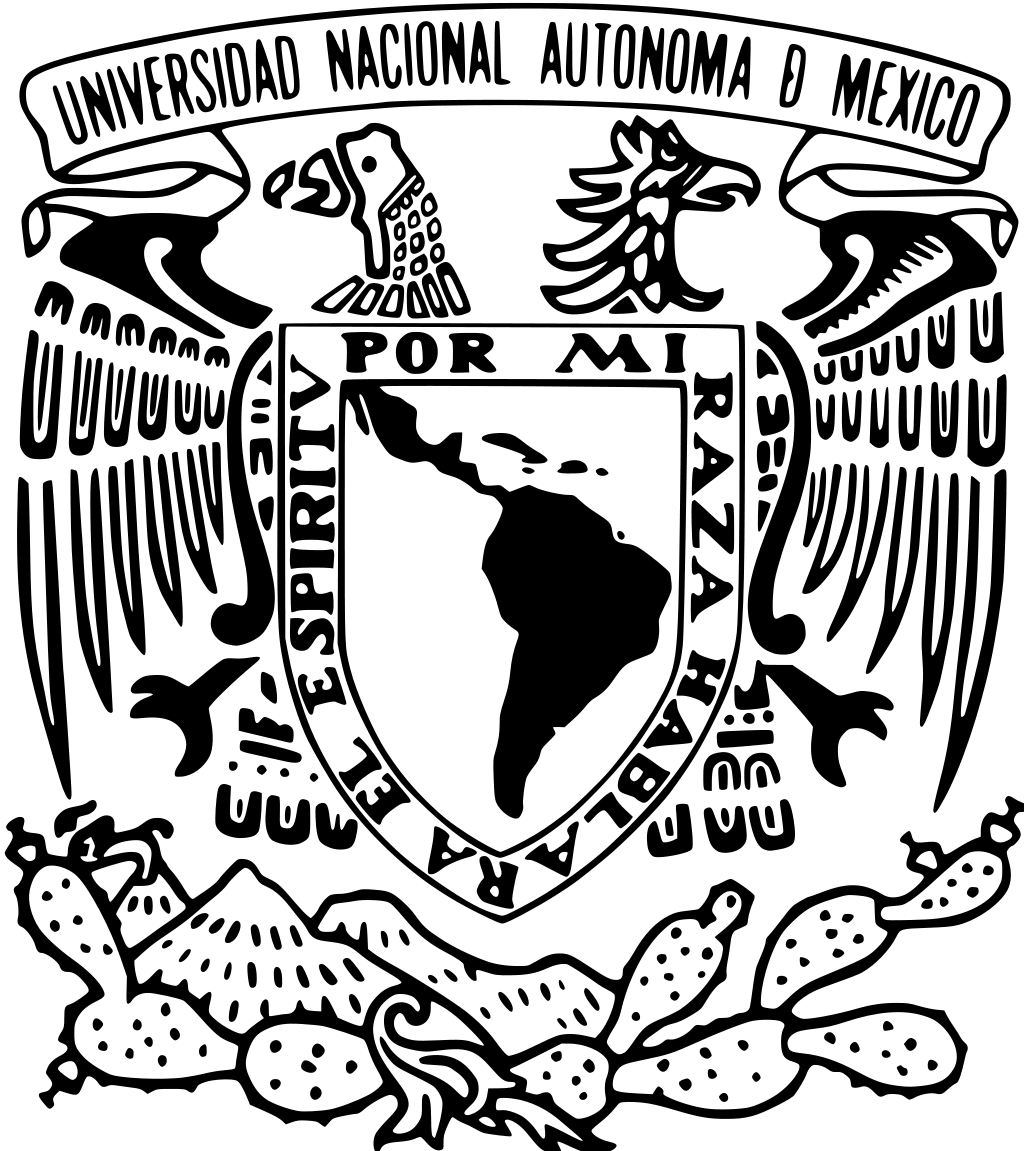
\includegraphics[width=0.2\textwidth]{../unam.png}
        \vspace*{.5cm}

        \LARGE
        \textbf{Universidad Nacional Autónoma de México}

        \vspace{0.5cm}
        \LARGE
        Facultad de Estudios Superiores Acatlán

        \vspace{2cm}

        \textbf{Apuntes} \\
        Ecuaciones Diferenciales

        \vfill

        \vspace{1cm}

        \textbf{\large Autor:} \\
        Jorge Miguel Alvarado Reyes \\
        \vspace{.5cm}
        \normalsize \today

    \end{center}
\end{titlepage}
\newpage

\tableofcontents

\newpage

\section{30/01/2024}

\subsection{Contacto}

\begin{itemize}
    \item Email: Camo6812@acatlan.unam.mx
\end{itemize}

\subsection{Evaluación}

\begin{itemize}
    \item Tareas 60\% Examenes 40\%
\end{itemize}

\textbf{Tarea}

Tomarse una selfi con una de las referencias bibliograficas

\section{01/02/2024}

\subsection{Transformadas integrales}

Las transformadas integrales son operadores que asocian nuevas funciones a un determinado conjunto mediante integración respecto a un determinado parámetro. La forma general de una transformada integral se puede expresar como:

\[
    T\{f(t)\} = F(s) = \int_{a}^{b} K(s, t) f(t) \, dt
\]

Donde:
\begin{itemize}
    \item $T$ representa el operador de transformada.
    \item $f(t)$ es la función original que queremos transformar.
    \item $F(s)$ es la función transformada, que depende de la variable $s$.
    \item $K(s, t)$ es el núcleo de la transformada, una función que depende tanto de la variable original $t$ como de la nueva variable $s$.
    \item $a$ y $b$ son los límites de integración, que pueden ser finitos o infinitos dependiendo del tipo específico de transformada integral.
\end{itemize}

Las transformadas integrales más conocidas y utilizadas incluyen:

\begin{itemize}
    \item \textbf{La Transformada de Fourier}, donde $a = -\infty$, $b = \infty$, y $K(s, t) = e^{-2\pi ist}$, utilizada ampliamente en el análisis de señales y sistemas.
    \item \textbf{La Transformada de Laplace}, con $a = 0$, $b = \infty$, y $K(s, t) = e^{-st}$, muy usada en la solución de ecuaciones diferenciales y en la teoría de control.
    \item \textbf{La Transformada de Mellin}, que es otra forma de transformada integral con un núcleo específico que permite transformaciones de productos en convoluciones, útil en teoría de números y análisis complejo.
\end{itemize}

Estas transformadas convierten funciones del dominio del tiempo o espacio (dominio $t$) a funciones en el dominio de frecuencias o complejo (dominio $s$), facilitando la manipulación matemática y la solución de problemas complejos.

\vspace{.25cm}

\textbf{Tarea 2}

En \url{https://es.wikipedia.org/wiki/Transformada_integral} hay una tabla con las tranformaciones y sus inversas. Elabore una tabla similar pero con nuestra simbologia. Para cada tranformada intente calcular la de $f(t) = t + c$

\[
    \lim_{\substack{a \to -\infty \\ b \to \infty}} \int_{a}^{b} \frac{1}{\pi}\left(\frac{1}{s-c-t}\right) \, dt
\]

\[
    \lim_{\substack{a \to -\infty \\ b \to \infty}}  \frac{1}{\pi} \int_{a}^{b} \left(\frac{1}{s-c-t}\right) \, dt
\]

\[
    \lim_{\substack{a \to -\infty \\ b \to \infty}}  \frac{1}{\pi} \int_{a}^{b} \left(\frac{1}{u}\right) - \, du
\]

\[ \lim_{\substack{a \to -\infty \\ b \to \infty}}  \frac{1}{\pi} - \left[\ln(u)\right]_{a}^{b}\]

\textbf{Ejercicios}

La tranformada de Laplace y condiciones de existencia

Para calcular la transformada de Laplace de \(f(t) = \sin(t)\), utilizamos la definición:
\[
    \mathcal{L}\{\sin(t)\} = \int_{0}^{\infty} e^{-st} \sin(t) \, dt
\]

Aplicamos la técnica de integración por partes, donde elegimos:
\begin{align*}
    u  & = \sin(t),    & dv & = e^{-st} dt                            \\
    du & = \cos(t) dt, & v  & = \int e^{-st} dt = -\frac{1}{s}e^{-st}
\end{align*}

La fórmula de integración por partes \(\int u dv = uv - \int v du\) nos lleva a:
\[
    \int_{0}^{\infty} e^{-st} \sin(t) \, dt = \left[-\frac{1}{s} \sin(t) e^{-st}\right]_{0}^{\infty} + \frac{1}{s} \int_{0}^{\infty} e^{-st} \cos(t) \, dt
\]

\[
    \int_{0}^{\infty} e^{-st} \sin(t) \, dt = 0 + \frac{1}{s} \int_{0}^{\infty} e^{-st} \cos(t) \, dt
\]

Ahora debemos calcular

\[
    \frac{1}{s} \int_{0}^{\infty} e^{-st} \cos(t) \, dt
\]

Aplicamos la técnica de integración por partes, donde elegimos:
\begin{align*}
    u  & = \cos(t),     & dv & = e^{-st} dt                            \\
    du & = -\sin(t) dt, & v  & = \int e^{-st} dt = -\frac{1}{s}e^{-st}
\end{align*}

\[
    \frac{1}{s} \int_{0}^{\infty} e^{-st} \cos(t) \, dt = \left[-\frac{1}{s} \cos(t) e^{-st}\right]_{0}^{\infty} + \frac{1}{s} \int_{0}^{\infty} e^{-st} - \sin(t) \, dt
\]

\[
    \frac{1}{s}\int_{0}^{\infty} e^{-st} \cos(t) \, dt = 0 + \frac{1}{s} \int_{0}^{\infty} e^{-st} - \sin(t) \, dt
\]

\[
    \frac{1}{s}\int_{0}^{\infty} e^{-st} \cos(t) \, dt =\frac{1}{s} \left(- \frac{1}{s} \int_{0}^{\infty} e^{-st} \sin(t) \, dt\right)
\]

\[
    \frac{1}{s}\int_{0}^{\infty} e^{-st} \cos(t) \, dt =\left(-\frac{1}{s^2} \int_{0}^{\infty} e^{-st} \sin(t) \, dt\right)
\]

\newpage

Para calcular la transformada de Laplace de \(f(t) = \cos(\alpha t)\), utilizamos la definición:
\[
    \mathcal{L}\{\cos(\alpha t)\} = \int_{0}^{\infty} e^{-st} \cos(\alpha t) \, dt
\]

Aplicamos la técnica de integración por partes, donde elegimos:
\begin{align*}
    u  & = \cos(\alpha t),         & dv & = e^{-st} dt           \\
    du & = -\alpha \sin(\alpha t), & v  & =  -\frac{1}{s}e^{-st}
\end{align*}

La fórmula de integración por partes \(\int u dv = uv - \int v du\) nos lleva a:

\begin{align*}
    \int_{0}^{\infty} \cos(\alpha t) e^{-st} \, dt & = \left[\cos(\alpha t) -\frac{1}{s}e^{-st}\right]_{0}^{\infty} - \int_{0}^{\infty} -\frac{1}{s}e^{-st} - \alpha \sin(\alpha t) \, dt
\end{align*}

\[\left[\cos(\alpha t) -\frac{1}{s}e^{-st}\right]_{0}^{\infty} = \left[\cos(\alpha \infty) -\frac{1}{s}e^{-s\infty} - \cos(\alpha 0) -\frac{1}{s}e^{-s 0}\right]\]

\[\left[\cos(\alpha \infty) -\frac{1}{s}e^{-s\infty} - \cos(\alpha 0) -\frac{1}{s}e^{-s 0}\right] = \frac{1}{s}\]

\begin{align*}
    \int_{0}^{\infty} \cos(\alpha t) e^{-st} \, dt & = \frac{1}{s} - \frac{\alpha}{s} \int_{0}^{\infty} e^{-st}  \sin(\alpha t) \, dt
\end{align*}

Debemos resolver

\[ \int_{0}^{\infty} e^{-st} \sin(\alpha t) \, dt\]

Aplicamos la técnica de integración por partes, donde elegimos:
\begin{align*}
    u  & = \sin(\alpha t),        & dv & = e^{-st} dt           \\
    du & = \alpha \cos(\alpha t), & v  & =  -\frac{1}{s}e^{-st}
\end{align*}

\begin{align*}
    \int_{0}^{\infty} \sin(\alpha t) e^{-st} \, dt & = \left[ \sin(\alpha t) \cdot -\frac{1}{s}e^{-st}\right]_{0}^{\infty} - \int_{0}^{\infty} -\frac{1}{s}e^{-st} \cdot \alpha \cos(\alpha t)
\end{align*}

\[\left[ \sin(\alpha t) \cdot -\frac{1}{s}e^{-st}\right]_{0}^{\infty} = \left[\sin(\alpha \infty) \cdot -\frac{1}{s}e^{-s\infty} - \sin(\alpha 0) \cdot -\frac{1}{s}e^{-s0}\right] = 0\]

\begin{align*}
    \int_{0}^{\infty} \sin(\alpha t) e^{-st} \, dt & = 0 - \int_{0}^{\infty} -\frac{1}{s}e^{-st} \cdot \alpha \cos(\alpha t) \\
                                                   & = \frac{\alpha}{s} \int_{0}^{\infty} e^{-st} \cos(\alpha t)
\end{align*}

\section{08/02/2024}

\subsection{Teoremas de la tranformada de laplace}

\[
    \mathcal{L}\{c\} = \frac{c}{s}
\]

\[
    \mathcal{L}\{t^n\} = \frac{n!}{s^{n+1}}
\]

\[
    \mathcal{L}\{sen(\alpha t)\} = \frac{\alpha}{s^2 + \alpha^2}
\]

\[
    \mathcal{L}\{cos(\alpha t)\} = \frac{s}{s^2 + \alpha^2}
\]

\[
    \mathcal{L}\{e^{\alpha t}\} = \frac{1}{s - \alpha}
\]

\[
    \mathcal{L}\{senh(\alpha t)\} = \frac{\alpha}{s^2 - \alpha^2}
\]

\[
    \mathcal{L}\{cosh(\alpha t)\} = \frac{s}{s^2 - a^2}
\]

\newpage

\section{Tarea 4}

\begin{enumerate}
    \item $y' + 4y = e^{-4t}, \hspace{.5cm} y(0) = 2$
    \item $y' - y = 1 - te^{t}, \hspace{.5cm} y(0) = 0$
    \item $y'' + 2y' + y = 0, \hspace{.5cm} y(0) = y'(0) = 1$
    \item $y'' - 4y' + 4y = t^{3}e^{2t}, \hspace{.5cm} y(0) = y'(0) = 0 $
    \item $y'' - 6y' + 9y = t, \hspace{.5cm} y(0) = 0, y'(0) = 1$
    \item $y'' - 4y' + 4y = t^3, \hspace{.5cm} y(0) = 1, y'(0) = 0 $
    \item $y'' - 6y' + 13y = 0, \hspace{.5cm} y(0) = 0, y'(0) = -3$
    \item $2y'' + 20y' + 51y = 0, \hspace{.5cm} y(0) = 2, y'(0) = 0$
    \item $y'' - y' = e^{t}cos(t), \hspace{.5cm} y(0) = 0, y'(0) = 0 $
    \item $y'' - 2y' + 5y = 1 + t, \hspace{.5cm} y(0) = 0, y'(0) = 4$
\end{enumerate}

\newpage

\subsection{Solución}

\subsection*{Problema 1}
$y' + 4y = e^{-4t}, \hspace{.5cm} y(0) = 2$

La Transformada de Laplace de la ecuación es:
\begin{equation}
    \mathcal{L}\{y'\} + 4\mathcal{L}\{y\} = \mathcal{L}\{e^{-4t}\}.
\end{equation}
\[
    \mathcal{L}\{e^{-4t}\} = \frac{1}{s + 4}.
\]
\[
    \mathcal{L}\{e^{-4t}\} = \int_0^\infty e^{-st}e^{-4t}\,dt.
\]
\[
    \mathcal{L}\{e^{-4t}\} = \int_0^\infty e^{-(s+4)t}\,dt.
\]
\[
    \mathcal{L}\{e^{-4t}\} = \left[ -\frac{1}{s+4}e^{-(s+4)t} \right]_0^\infty.
\]
Usando las propiedades de la Transformada de Laplace, tenemos:
\begin{align*}
    \mathcal{L}\{y'\} & = sY(s) - y(0), \\
    \mathcal{L}\{y\}  & = Y(s),
\end{align*}

Sustituyendo con la condicion inicial \(y(0) = 2\) en la ecuación:
\begin{equation}
    sY(s) - 2 + 4Y(s) = \frac{1}{s + 4}.
\end{equation}

Esto simplifica a:
\begin{equation}
    (s + 4)Y(s) = 2 + \frac{1}{s + 4}.
\end{equation}

Despejamos \(Y(s)\):
\begin{equation}
    Y(s) = \frac{2}{s + 4} + \frac{1}{(s + 4)^2}.
\end{equation}

Para encontrar \(y(t)\), aplicamos la Transformada de Laplace inversa a \(Y(s)\), usando las transformadas inversas conocidas:
\begin{equation}
    y(t) = 2e^{-4t} + te^{-4t}.
\end{equation}

Este es el resultado de aplicar la Transformada de Laplace y su inversa a la ecuación diferencial dada, con la condición inicial \(y(0) = 2\).

\subsection*{Problema 4}
$y'' - 4y' + 4y = t^{3}e^{2t}, \hspace{.5cm} y(0) = y'(0) = 0 $

Aplicamos la Transformada de Laplace a ambos lados de la ecuación:
\begin{equation}
    \mathcal{L}\{y''\} - 4\mathcal{L}\{y'\} + 4\mathcal{L}\{y\} = \mathcal{L}\{t^3e^{2t}\}.
\end{equation}

Utilizamos las propiedades de la Transformada de Laplace para las derivadas y la condición inicial dada:
\begin{align*}
    \mathcal{L}\{y'\}  & = sY(s) - y(0),            \\
    \mathcal{L}\{y''\} & = s^2Y(s) - sy(0) - y'(0).
\end{align*}

Dado que \(y(0) = y'(0) = 0\), simplificamos a:
\begin{align*}
    \mathcal{L}\{y'\}  & = sY(s),   \\
    \mathcal{L}\{y''\} & = s^2Y(s).
\end{align*}

Para calcular \(\mathcal{L}\{t^3e^{2t}\}\), aplicamos el teorema del desplazamiento en el eje \(s\) y obtenemos:
\begin{equation}
    \mathcal{L}\{t^3e^{2t}\} = \frac{3!}{(s-2)^4} = \frac{6}{(s-2)^4}.
\end{equation}

Sustituimos estos resultados en la ecuación transformada:
\begin{equation}
    s^2Y(s) - 4sY(s) + 4Y(s) = \frac{6}{(s-2)^4}.
\end{equation}

Factorizamos el término en \(Y(s)\) y simplificamos:
\begin{equation}
    Y(s)(s^2 - 4s + 4) = \frac{6}{(s-2)^4},
\end{equation}
\begin{equation}
    Y(s)(s - 2)^2 = \frac{6}{(s-2)^4}.
\end{equation}

Finalmente, despejamos \(Y(s)\):
\begin{equation}
    Y(s) = \frac{6}{(s-2)^6}.
\end{equation}

Este resultado representa la Transformada de Laplace de la solución \(y(t)\) de la ecuación diferencial original. Para encontrar \(y(t)\), aplicaríamos la Transformada de Laplace inversa a \(Y(s)\).


\end{document}